\documentclass[tikz,border=10pt]{standalone}
\begin{document}
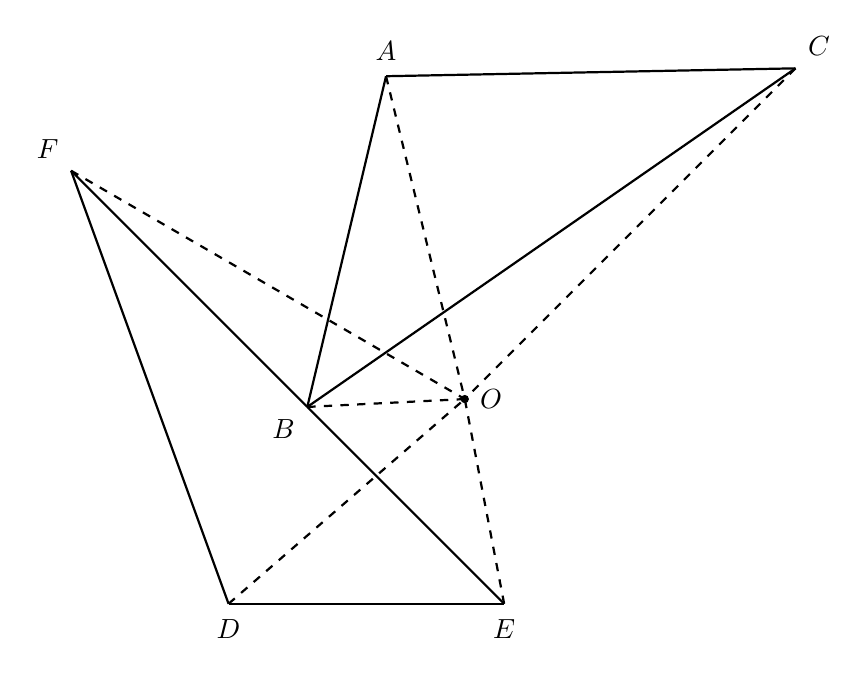
\begin{tikzpicture}[scale=1]
  \coordinate (A) at (0,6.2);
  \coordinate (C) at (5.2,6.3);
  \coordinate (B) at (-1,2);
  \coordinate (O) at (1,2.1);
  \coordinate (F) at (-4,5);
  \coordinate (D) at (-2,-0.5);
  \coordinate (E) at (1.5,-0.5);

  % solid edges
  \draw[thick] (A) -- (C);
  \draw[thick] (A) -- (B);
  \draw[thick] (B) -- (C);
  \draw[thick] (F) -- (D);
  \draw[thick] (F) -- (B);
  \draw[thick] (B) -- (E);
  \draw[thick] (D) -- (E);

  % dashed edges
  \draw[dashed,thick] (A) -- (O);
  \draw[dashed,thick] (C) -- (O);
  \draw[dashed,thick] (B) -- (O);
  \draw[dashed,thick] (D) -- (O);
  \draw[dashed,thick] (E) -- (O);
  \draw[dashed,thick] (F) -- (O);

  % labels
  \node[above=2pt] at (A) {$A$};
  \node[above right=1pt] at (C) {$C$};
  \node[below left=1pt] at (B) {$B$};
  \node[right=2pt] at (O) {$O$};
  \node[above left=1pt] at (F) {$F$};
  \node[below=2pt] at (D) {$D$};
  \node[below=2pt] at (E) {$E$};

  \fill (O) circle (1.5pt);
\end{tikzpicture}
\end{document}
